\documentclass[dvips,dvipdfm,pdftex]{llncs}
\usepackage[utf8]{inputenc}
\usepackage{amsmath}
\usepackage{amsfonts}
\usepackage{amssymb}
\usepackage[dvips,dvipdfm,pdftex]{graphicx}
\usepackage{pgfplotstable}
\usepackage{array}
\usepackage{booktabs}
\usepackage{morefloats}
\usepackage{etex}
\usepackage{listings}
\usepackage{float}
\usepackage[section]{placeins}
\usepackage[ruled,linesnumbered,resetcount,algochapter]{algorithm2e}


\title{Semi-supervised Hidden Markov Random Fields (HMRF) Kmeans. Theory to Implementation\\}
\author{Dimitrios Pritsos and Efstathios Stamatatos}
\institute{University of the Aegean\\Karlovassi, Samos \textendash{} 83200, Greece.\\\{dpritsos, stamatatos\}@aegean.gr }

\begin{document}

\maketitle

\begin{abstrat}

\end{abstrat}


\section{Introduction}\label{sec:intro}
The objective of the Semi-supervised Clustering is to incorporate in the procedure of clusters discovery or assignment, the prior knowledge about the skeleton of the clusters schema. There are several efforts on Semi-supervised model inference in both Expectation Maximization (EM) clustering based models and in Agglomerating clustering based models. According to \cite{chapelle2006semi_hmrf_kmeans} there three main groups of EM based semi-supervised clustering methods:

\begin{enumerate}
	\item \emph{Constraints-based mehtods} are using the provided supervision for guiding the algorithm towards a data partitioning which is avoiding (but not prevening) the constraints violation.
	\item \emph{Distance-based approaches} in clustering method with a particular distance funciton; the distance function is parametrized and the parameters values are learned to satisfy the constraints.
	\item \emph{Semi-supervised clustering based on Hidden Markov Random Fields} where the constraint-based and distance-based approaches are combined into \emph{a unified probabilistic model}.
\end{enumerate}

In EM clustering based models there have been several efforts where the labeled data where provided in the clustering model in the form of data-labels pairs or in the initialization phase of theclustering model. In this work we present the Hidden Markov Random Fields Model(HMRF) Kmeans, where the prior knowledge about the structure or skeleton of the clusters schema has been embedded into the model in the form of constraints \cite{basu2004probabilistic}. The HMRF Kmeans is a hard-clustering model due to the \emph{hard} assignment of the data point to one of the a-priori fixednumber of clusters. However, the same models can be transformed into a relatively easy soft-clustering model where of each data point only Maximum a-posteriry Probability (MAP) of the point to bea member of each cluster of th final schema.

The HMRF Kmeans Semi-supervised clustering method it has been implemented, in this work, for being tested on the Web Genre Identification (WGI) Information Retrieval (IR) taxonomy problem.Therefore, here we only present the model inference procedure where the distance measure, a.k.a distortion function/measure, is the cosine similarity because in the IR literature is the distortionmeasure where in most cases maximizes performance in problems where the feature space is particularly large, as in this case. In case one would be interested in changing the model to asoft-clustering method then the probability destiny function of the final model should have been chosen to be some properly parametrized Von Mises Fisher distributions.

Since this work is focusing on the implementation of Semi-supervised HMRF-Kmeans in the IR domain framework, it has to be noted that this Semi-supervised model advantage is the interactivelearning setting where this model can be used \cite{chapelle2006semi_hmrf_kmeans}, since the constraints are provided to the model in two different sets the \emph{Must-Link} and\emph{Cannot-Link}. These sets are not necessarily the same in size or complimentary one to the other.

What it follows is the model inference line of thought based on the there resources \cite{basu2004probabilistic,chapelle2006semi_hmrf_kmeans,bishop2006_EM_general_view}.

\section{Model inference}\label{sec:model_inference}
The objective of a semi-supervised model like HMRF Kmeans is to drive the procedure of clustering schema taking into account the prior knowledge we have about the clusters in the form of\emph{must-link} and \emph{cannot-link} constraints. The main difference in the graphical model of a topical EM algorithm is the nodes of the observed labeled data over the hidden, a.k.a latent,variables as depicted in fig.\ref{fig:hmrf_em}, with red colored arrows and gray shaded nodes.

\begin{figure}[h]
	\begin{center}
		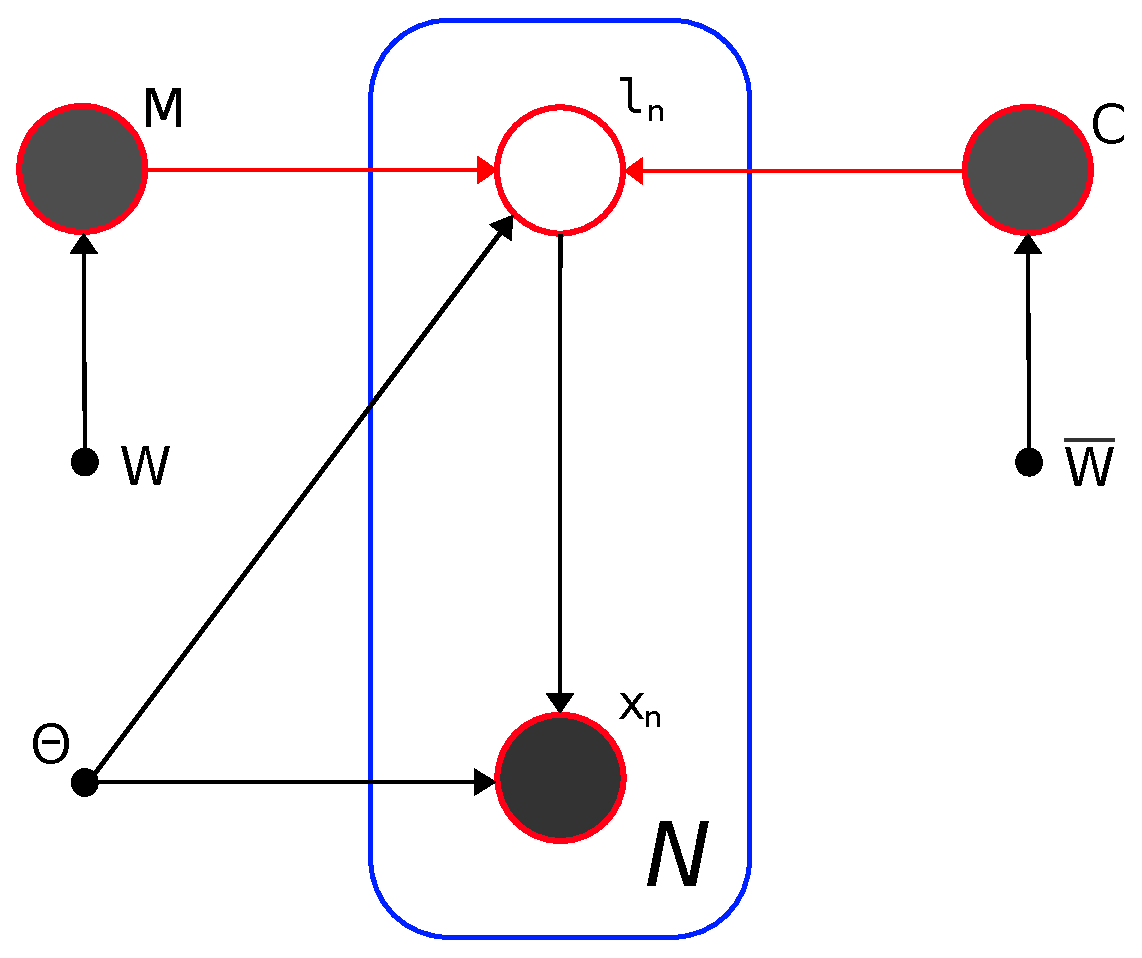
\includegraphics[scale=0.40]{figures/SemiSupervised_HMRF_EM_Graphical_Model.eps}
		\caption{Semi-supervised HMRF Expectation Maximization or Kmeans Clustering Graphical Model.}
		\label{fig:hmrf_em}
	\end{center}
\end{figure}

The goal of EM is to maximize the \emph{log likelihood function} $P(X|\Theta)$ with respect of $\Theta$ as in eq.\ref{eq:em_log_likelihood}.

\begin{equation}
lnP(X|\Theta)=ln\left\{ \sum_{l}P(X,L|\Theta)\right\}
\label{eq:em_log_likelihood}
\end{equation}

Where $X=\{\mathbf{x}_{i}\}_{i=1}^{N}$ is the set of \emph{observable random variables} given by the conditional probability $P(X|\Theta)$ and $\mathbf{x}_{i}$ is a random vector (or data point) of the corpus under taxonomy. Note the boldface notation of the random vector in order not to be mixed with $x_{i}$ which will a feature (or variable) of this vector. Moreover, $N$ is the number of vector as depicted in the graphical model of fig.\ref{fig:hmrf_em}.

Due to the relatively complex marginal distributions, like $P(X|\Theta)$, over observed data points where they are computationally intractable, there is a common practice to incorporate \emph{latent or hidden variables} in order to express the conditional probability calculation more tractable over the expanded space of observed and latent variables. In eq.\ref{eq:em_log_likelihood} $L$ is the set of hidden (or latent) variables over $X$ observable data points \cite{bishop2006_EM_general_view}.

Therefor \emph{a hidden field} $L=\{\mathbf{l}_{i}\}_{i=1}^{N}$ random variables, \emph{whose values are unobservable}. In the clustering framework, the set of hidden variables are the unobserved cluster labels on the
points, indicating cluster assignments. Every hidden variable $\mathbf{l}_{i}$ takes values from the set ${1, . . . , N}$, which are the labels of the clusters.

Now every random data point $\mathbf{x}$ can be generated from a conditional probability distribution $P(\mathfb{x}_{i}|\mathbf{l}_{i})$ determined by the corresponding hidden variable $\mathbf{l}_{i}$. Note that we know a-priory that the random data points $X$ are conditionally independent given the hidden variables $L$. Thus $P(X|L) = \prod_{\mathbf{x}_{i} \in X}P(\mathbf{x}_{i}|\mathbf{l}_{i})$. Note that $\mathbf{l}_{i}$ can be either a vector or a singleton depending on the algorithm setting, either for soft-clustering or for hard-clustering respectively. Thus value and vector for $\mathbf{l}_{i}$ will be used interchangeably in this text.

The set of $\left\{X,Z\right\}$ is \emph{the complete data set}, while the $\left\{X\right\}$ is \epmh{the incomplete data set}. The likelihood function for the complete data set simply takes the form $lnp(X,Z|\Theta)$ as shown in eq.\ref{eq:em_log_likelihood}, and theoretically that maximization of this complete data log likelihood function is straightforward. However, in practice we are not given the complete data set, but only the incomplete data points $X$. Thus, our only knowledge of for the values of the latent (hidden) variables in $L$ is given by the posterior distribution $p(Z|X,\Theta)$. Because we don't have available the complete-data log likelihood, we consider instead its expected value under the posterior distribution of the latent (hidden) variables.

In eq.\ref{eq:em_log_likelihood} and in fig.\ref{fig:hmrf_em} there are some parameters $\Theta$ which are governing the initial and the final schema of the PDF's mixture. These are the parameters we have to find computationally and where in employee EM algorithm (alg.\ref{alg:em_generic}) with the following general and distribution inexpedient (i.e. irrespectively where the PDF's are Gaussian, Von Mises Fisher etc). In particular with EM we are interactively finding the proper set of $\Theta$ parameters by calculating the expected posterior distribution $P(L|X,\Theta)$ of the latent (hidden) variables $L$.

\begin{algorithm}[H]\label{alg:em_generic}
\KwData{\\
		\hspace{.01\textwidth} $\mathbf{X}$ observable data points.\\
		\hspace{.01\textwidth} $\mathbf{K}$ possible states clusters we expect to be existing in the data-set.\\
		\hspace{.01\textwidth} $\mathbf{L}_{i=1}^K$ the hidden field variables (or vectors) with values $\left\{1,...,\mathbf{K}\right\}$ or $(0,1]$\\
		\hspace{.01\textwidth} $\mathbf{\Theta}$ an initial state about the PDF mixture model.\\
		}
\KwResult{\\
		  \hspace{.01\textwidth} $\mathbf{l} = \{\mathbf{p}_{k}\}_{k=1}^{K}$ where $\mathbf{p}$ can be either $\left\{0,1\right\}$ or $(0,1]$
 		  depending on the soft-clustering of hard-clustering set-up.\\
		  \hspace{.01\textwidth} $\mathbf{\Theta}$ the final set of parameters after the Probability Density Functions Mixture.
		 }
Choose an Initial setting for $\mathbf{\Theta}^{OLD}$;\\
\While{$I$ iterations not reached}{
	\textbf{1. E-step }Evaluate $P(\mathbf{L}|\mathbf{X},\mathbf{\Theta}^{OLD})$\;\\
	\textbf{2. M-step }Evaluate $\mathbf{\Theta^{NEW}}$\ given by (a) and (b);\\
	\hspace{.1\textwidth} \textbf{a.} $\mathbf{\Theta}^{NEW}=\arg_{\mathbf{\Theta}}\max\Omega(\mathbf{\Theta},\mathbf{\Theta}^{OLD})$\;\\
	\hspace{.1\textwidth} \textbf{b.} $\Omega(\mathbf{\Theta},\mathbf{\Theta}^{OLD})=\sum_{\mathbf{L}}P(\mathbf{L|X},\mathbf{\Theta}^{OLD})lnP(\mathbf{X,L},\mathbf{\Theta})$\;\\

	\eIf{log likelihood convergence reached}{
		Breaking the loop and Ending the Clustering\;
	}{
		$\mathbf{\Theta}^{OLD}\leftarrow\mathbf{\Theta}$\;
	}
}

\caption{The generic for of Expectation Maximization either for both Soft- and Hard-clustering }
\end{algorithm}

The EM algorithm can also be used to find MAP (maximum a-posterior) solutions in case we have a good knowledge about the prior distribution $P(\mathbf{\Theta})$ over the parameters $\mathbf{\Theta}$. In this case the E-step remains the same as in the maximum likelihood case, while in the \emph{M-step (b)} the $\Omega(\mathbf{\Theta},\mathbf{\Theta}^{OLD})+lnP(\mathbf{\Theta})$.

\textbf{In HMRF-Kmeans derivation process} we are starting with the PDF mixture we would like to maximize by exploring the EM for the reasons explained above, as shown in eq.\ref{eq:hmrm_em_pdf}.

\begin{equation}
	P(\mathbf{X,L,\Theta}|\mathbf{M,C})=P(\mathbf{\Theta}|\mathbf{M,C})P(\mathbf{L}|\mathbf{\Theta,M,L})P(\mathbf{X}|\mathbf{L,\Theta,M,C})
\label{eq:hmrm_em_pdf}
\end{equation}

Where the set of vector are the same as in alg.\ref{alg:em_generic} but this time the constraints set of the fig.\ref{fig:hmrf_em} have been included, i.e. Mast-link and Cannot-link constraints set $\left\{\mathbf{M,C}\right\}$. Moreover, as the graphical model is describing the constraints are independent from $\mathbf{X}$ and parameters $\mathbf{\Theta}$ are, also, independent from the constraints set. Thus:

\begin{equation}
	P(\mathbf{X}|\mathbf{L,\Theta,M,C})=P(\mathbf{X}|\mathbf{L,\Theta})
\label{eq:hmrm_em_X_MC_interdependency}
\end{equation}

\begin{equation}
	P(\mathbf{\Theta}|\mathbf{M,C})=P(\mathbf{\Theta})
\label{eq:hmrm_em_Theta_MC_interdependency}
\end{equation}

Considering $\mathbf{X}$ observable data-set is convient due to compuational issues to simplify the algorithm by assuming the vectors $\mathbf{x}$ are \emph{mutually impediment}, thus:

\begin{equation}
	P(\mathbf{X}|\mathbf{L,\Theta})=\prod_{i=1}^{N}P(\mathbf{x}_{i}|\mathbf{l}_{i},\mathbf{\Theta})
\label{eq:hmrm_em_X_mutually_interdependency}
\end{equation}

Consequentially, from equations \ref{eq:hmrm_em_pdf}, \ref{eq:hmrm_em_X_MC_interdependency}, \ref{eq:hmrm_em_Theta_MC_interdependency} and \ref{eq:hmrm_em_X_mutually_interdependency} we are getting the following MAP which it should be maximized.

\begin{equation}
	P(\mathbf{X,L,\Theta}|\mathbf{M,C})=P(\mathbf{\Theta})P(\mathbf{L}|\mathbf{\Theta,M,C})\prod_{i=1}^{N}P(\mathbf{x}_{i}|\mathbf{l}_{i},\mathbf{\Theta})
\label{eq:hmrm_em_MAP_or_MAX_Liklihood}
\end{equation}

At this step of the clustering method building process we have to decide weather the clustering would be soft or hard. This decision has two consequences. Firstly, is related to the $\mathbf{L}$ latent variables type and range of values as shown in alg.\ref{alg:em_generic}, i.e. whether $\mathbf{l}$ will be a variable or a vector of variables and whether its values will be probability estimates or {0,1} depending whether of not a data-point is belonging to the cluster $\mathbf{k}_{i}$. Secondly, is related whether the algorithm will be probabilistic based or distance based, i.e. whether a MAP will be maximized or an objective function with a specific distance measure (a.k.a distortion function/measure) will be minimized.

In our case go for the \emph{distortion function} path, as the Kmeans term of the algorithm implies. As explained above since we are focusing on IR domain problems we are going to show the complete algorithm building process for the cosine similarity as the distortion function of our choice.

Each hidden random variable $\mathbf{l}_i$ has an associated set of neighbors $\mathbf{\Gamma}_{i}\subset\mathbf{L}$. The must-link and cannot-link constraints define the neighborhood over the hidden labels, such that the neighbors of a point $x_{i}$ are all points that must-linked and/or cannot-inked with. The \emph{random field defined over the hidden variables} is a \emph{Markov Random Field}, where the PDF of the hidden variables \emph{obeys the following Markov property}:

\begin{equation}
	\forall i,P(\mathbf{l}_{i}|\mathbf{L-}\{\mathbf{l}_{i}\},\mathbf{\Theta},\mathbf{M},\mathbf{C})=P(\mathbf{l}_{i}|\{\mathbf{\Gamma}_{i},\mathbf{\Theta},\mathbf{M},\mathbf{C}\})
\label{eq:markov_property}
\end{equation}

Therefore, the probability distribution of $\mathbf{l}$ labels is only dependent on the must-link and cannot-link constraints on $\mathbf{x}$ data-points. The above paragraph justifies the name for the algorithm as HMRF and letting us assume any a-piory PDF for an arbitrary label setup.

Since, by the \emph{Hammersley-Clifford theorem}, the a-prior PDF of a particular label setup can be expressed as a Gibbs distribution eq.\ref{eq:constraints_Gibbs_pdf}, which conveniently belongs to the exponential distributions family, as we will see later.

\begin{equation}
	P(\mathbf{L}|\mathbf{\Theta},\mathbf{M},\mathbf{C})=\frac{1}{Z_{1}}\exp(-\sum_{\mathbf{\Gamma}_{i}\in\Gamma}V_{\Gamma_{i}}(\mathbf{L}))
\label{eq:constraints_Gibbs_pdf}
\end{equation}

Where $V_{\Gamma_{i}}$ is the \emph{potential function}, as it called when the clustering model is \emph{hard} type \textbf{(NOTE: Potential Function also found this in the Bishops Book and I think this term is used in Kmeans case and not in the probabilistic EM)}, for each neighborhood of labels defined by the $\{M,C\}$ sets of constraints.

Since the constraints should probably been given as pairs then eq.\ref{eq:constraints_Gibbs_pdf} will become eq.\ref{eq:constraints_Gibbs_pdf_pairwise}.\textbf{(NOTE:A question here is constraint A=(2,50) will be the same as B=(50,2), will both be present etc. Should the constraints be a Graph, a Matrix or a set of pairs? (Impementation Language Performance VS Math/Computational Performance))}.

\begin{equation}
	P(\mathbf{L}|\mathbf{\Theta},\mathbf{M},\mathbf{C})=\frac{1}{Z_{1}}\exp(-\sum_{i}\sum_{j}V(i,j))
\label{eq:constraints_Gibbs_pdf_pairwise}
\end{equation}

\begin{equation}
	V(i,j)=
	\begin{cases}
		f_{\mathbf{M}}(x_{i},x_{j}) & \text{if }(x_{i},x_{j})\in\mathbf{M}\\
		f_{\mathbf{C}}(x_{i},x_{j}) & \text{if }(x_{i},x_{j})\in\mathbf{C}\\
		0 & \text{otherwise}
	\end{cases}
\label{eq:constraints_potential_function}
\end{equation}

Where $f_{\mathbf{M}}$ and $f_{\mathbf{C}}$ are positive value cost functions for the must-link and cannot-link constraints violation. Clearly, eq.\ref{eq:constraints_Gibbs_pdf_pairwise} is discouraging the violation of the constraints by reducing the value of joint probability MAP in eq.\ref{eq:hmrm_em_MAP_or_MAX_Liklihood}.

Maximizing the joint HMRF probability in eq.\ref{eq:hmrm_em_MAP_or_MAX_Liklihood} (left part of the equation), is equivalent to jointly maximizing the likelihood of generating data points from the model and the probability of label assignments that respect the constraints, while regularizing the model parameters. The essential part of the right side of the equation the conditional probability $P(\mathbf{X}|\mathbf{L},\mathbf{M},\mathbf{C})$, equivalent to eq.\ref{eq:hmrm_em_X_MC_interdependency}. Firstly, because its PDF will define our prior assumption about the PDF mixture of the data-set. Secondly, because the same PDF should be used as the constraints potential function $V$, thus, penalty functions $f$. Finally, because its PDF will ultimately define the parametrized (by $\Theta$ parameters) \emph{distortion measure}.

Using the convenience in the assumption of a regular exponential distributions for the observed data points $X$ and a regular Bregman divergences, the PDF of the observed data would be in eq.\ref{eq:PDF_with_distortion_measure}.

\begin{equation}
	P(\mathbf{x}_{i}|\mathbf{l}_{i},\mathbf{\Theta})=\frac{1}{Z_{2}}\exp(-D_{\mathbf{A}}(x_{i},\mathbf{\mu}_{\mathbf{l}_{i}}))
\label{eq:PDF_with_distortion_measure}
\end{equation}

where $D_{\mathbf{A}}(\mathbf{x}_{i} , \mathbf{x}_{\mathbf{l}_{i}})$ is the Bregman divergence, i.e. distortion measure, between $\mathbf{x}_i$ and $\mathbf{\mu}_{\mathbf{l}_{i}}$. Where $\mathbf{l}_i$ is indicating that the distance is measured for an arbitrary $\mathbf{x}_{i}$ is from the cluster centroid (or cluster's PDF expected value) when the point and the centroid a under the same cluster PDF \textbf{(NOTE: This is my conclusion and no one in literature give any specification related to the $\mu$ notation)}. $Z_{2}$ is the normalizing term (a.k.a \emph{partition function}).

As explained above in general EM algorithm description, we are at the step where we have to assume the PDF mixture of the observable data. In the semi-supervised case the a-piori distribution assumption will be the same, over the observable data-set $\mathbf{X}$ and the observable constraints sets $\mathbf{M,C}$. Thus, in our case, for the IR problems based on the literature, we assume for both the data-set and the constraints sets von-Mises Fisher (vMF) distribution with unit concentration parameter, which is equivalent to the spherical Gaussian distribution \cite{basu2004probabilistic,chapelle2006semi_hmrf_kmeans}. In order to make PDF of eq.\ref{eq:PDF_with_distortion_measure} to be equivalent to vMF the distortion parameter $D_{\mathbf{A}}$ will be replaced with the \emph{parametrized cosine distance} as defined in eq.\ref{eq:parametrized_cos_sim} by the parameters matrix $\mathbf{A}$.

\begin{equation}
	D_{cos_{\mathbf{A}}}(\mathbf{x}_{i},\mathbf{x}_{j})=\frac{\mathbf{x}_{i}^{T}\mathbf{A}\mathbf{x}_{j}}{\Vert\mathbf{x}_{i}\Vert_{\mathbf{A}}\Vert\mathbf{x}_{j}\Vert_{\mathbf{A}}}
	\label{eq:parametrized_cos_sim}
\end{equation}

Where $\Vert\mathbf{x}_{i}\Vert_{\mathbf{A}}=\sqrt{\mathbf{\mid x}_{i}^{T}\mathbf{A}\mathbf{x}_{j} \mid}$, \textbf{(NOTE: In \cite{basu2004probabilistic} under square root there is no norm, but in practice the product sometimes drops under zero and breaks the code run.)}

In the eq.\ref{eq:hmrm_em_MAP_or_MAX_Liklihood} (right side of the equation) we have defined the conditional probabilities for the observed $X$ and the $L$, where the second is conditioned under the constraints ${M,C}$. The presence of the $P(\mathbf{\Theta})$ is occurring due to the explicit presence of the joint distribution in eq.\ref{eq:hmrm_em_MAP_or_MAX_Liklihood} (left side of the equation) and the graphical model in fig.\ref{fig:hmrf_em}. This is enabling us to decide whether or not we want to apply our a-piori knowledge about the distribution of the parameters. This can be omitted when $\mathbf{\Theta}$ parameters are not explicitly present, as in \cite{basu2004probabilistic}, thus no prior assumptions about the parameters distribution is required or can be applied.

Depending on the prior distribution, parameters $\mathbf{\Theta}$ are separated in two sets $\mathbf{\Theta}=\{\mathbf{A},\mathbf{M}\}$, where the second one is the expected values of the mixture's PDF(s) and $\mathbf{A}$ is the rest of the required parameters.

\begin{equation}
	P(\mathbf{\Theta})=P(\mathbf{A})P(\mathbf{Mu})
\label{eq:ptheta}
\end{equation}


\subsection{Putting all together}

The objective of the semi-supervised HMRF Kmeans is to maximize the MAP as defined in eq.\ref{eq:hmrm_em_MAP_or_MAX_Liklihood} with the parts of this equation to be analyses in eq.\ref{eq:constraints_Gibbs_pdf} eq.\ref{eq:constraints_Gibbs_pdf} and eq.\ref{eq:ptheta} . Putting all these equations together we have eq.\ref{eq:final_MAP}.

\begin{equation}
	P(\mathbf{X,L,\Theta}|\mathbf{M,C})=P(\mathbf{A})P(\mathbf{Mu})(\frac{1}{Z_{1}}\exp(-\sum_{\mathbf{\Gamma}_{i}\in\Gamma}V_{\Gamma_{i}}(\mathbf{L})))\prod_{i=1}^{N}\frac{1}{Z_{2}}\exp(-D_{\mathbf{A}}(x_{i},\mathbf{\mu}_{\mathbf{l}_{i}}))
\label{eq:final_MAP}
\end{equation}

Our early decision was the hard-clustering setup for the algorithm thus my explaining the logarithmic properties from eq.\ref{eq:final_MAP} we are getting eq.\ref{eq:MAP_to_Objective}.

\begin{equation}
	\begin{split}
		\ln P(\mathbf{X,L,\Theta}|\mathbf{M,C})=\sum_{\mathbf{\Gamma}_{i}\in\Gamma}V_{\Gamma_{i}}(\mathbf{L})+\sum_{i=1}^{N}D_{\mathbf{A}}(x_{i},\mathbf{\mu}_{\mathbf{l}_{i}})+ \\
		\ln Z_{1}+N\ln Z_{2}-\ln P(\mathbf{A})-\ln P(\mathbf{Mu})
	\end{split}
\label{eq:MAP_to_Objective}
\end{equation}

Equation eq.\ref{eq:MAP_to_Objective} is now called the \emph{Objective Function} and the goal of the algorithm is to minimize its output, which is equivalent to the MAP maximization. Expressing it in words the minimization process of eq.\ref{eq:MAP_to_Objective} is equivalent to the the iterative process in order to find the proper clustering configuration where each arbitrary data-point is the closest to the mean value of the cluster it will belong into at the end. Moreover, the constraints violation will also be minimized. \textbf{(NOTE: Applying the logarithm on eq.\ref{eq:final_MAP} seems to me that all the sights in the right part of eq.\ref{eq:MAP_to_Objective} should have been exactly the opposite but in literature is not. Am I missing something here?)}

Before we proceed in replacing the exact violation $V$ and distortion measure $D$ functions with the parameterized cosine similarity we are considering the rest of the equation starting with the normalizing components $Z_{1}$ and $Z_{2}$. In additions to consider the distributions of the PDF mixture parameters $\mathbf{A}$ and $\mathbf{Mu}$.

The normalizing components of observable data points and the hidden variables distributions are depended on the prior PDF assumption. In case of Gaussian distribution their value can be calculated in a \emph{closed form} \textbf{(NOTE:No sure what exactly that is)} while for all the other case we have to employee an \emph{approximation method}. In our case where cosine similarity must be used an approximate inference method is required which can be very expensive computationally. In this case we can assume that $Z_{1}$ and $Z_{2}$ are constants. Now eq.\ref{eq:MAP_to_Objective} will no longer be an joint probability, however, empirically it has been shown that this objective functions will work properly and the algorithm will manage to converge in a local minimum \cite{basu2004probabilistic}. However, if in some applications it is important to preserve the joint probability model, then the normalizers should be estimated by approximate inference methods.

The distribution on cluster centroids $\{\mu_{i}\}_{i=1}^{K}$ can safely assumed to be uniformly distributed thus $P(\mathbf{Mu})$ can be assumed as constant, thus, $lnP(\mathbf{Mu})=0$. Distributions parameters $\mathbf{A}$ can lead to \emph{diegenerate solutions} of the optimization problem. As an example, for squared Euclidean distance it can be $\mathbf{A}=0$ as such solution. In order to prevent \emph{degenerate solutions}, $P(\mathbf{A})$ is used to regularize the parameter values using a prior distribution. In addition, we mostly need non-negative solutions for several computational problems might occur otherwise, thus, one such a distributions can be Rayleigh distribution as described in eq.\ref{eq:Rayleigh_pdf}, with the assumptions of mutually independent parameters values $\alpha$.

\begin{equation}
	P(\mathbf{A})=\prod_{\alpha_{ij}\in\mathbf{A}}\frac{\alpha_{ij}\exp(-\frac{\alpha_{ij}^{2}}{s^{2}})}{s^{2}}
\label{eq:Rayleigh_pdf}
\end{equation}

Where $s$ is the width parameter of the distortion.

The last step for deriving the Semi-supervised HMRF Kmeans is to define exactly the $f_{M}$ and $f_{C}$ sub-functions of the constraint violation $V$ functions of eq.\ref{eq:constraints_potential_function} based on the cosine similarity as explained above.

Starting with $f_{\mathb{M}}$, it should return the violation cost of must-link constrains between an $(i,j)$ pair if only $\mathbf{l}_{i} \neq \mathbf{l}_{j}$, i.e. their labels are not equal which means the are not belonging to the same cluster as they should. Moreover, we want to use the constraint violations to learn the underlying distance measure (distortion function), thus, the penalty for violating a must-link constraint between distant points should be higher than that between nearby points. Therefore, we have to adjust the distortion function to get there points closer as they should upon the must-link constraints. To do so we need the penalty scaling function to be a
monotonically increasing function of the distance between $x_i$ and $x_j$ according to the current distortion measure. Consequently, we have the following equation eq.\ref{eq:fm} which satisfies the above properties for $F_{M}$ \cite{basu2004probabilistic,chapelle2006semi_hmrf_kmeans} \textbf{(NOTE: The reasoning is very close but note exactly and I think my reasoning is more clear and more sensible, because theirs is a bit odd for example related to W, in Chappell's is better explained but more complex in notation. Also my notation defers allot because theirs finally is equivalent to my notation.)}.

\begin{equation}
	f_{\mathbf{M}}(x_{i},x_{j})=w_{ij}D_{cos_{\mathbf{A}}}\Psi(l_{i}\neq l_{j})
\label{eq:fm}
\end{equation}

The function $f_{\mathb{C}}$ for the cannot-link constraint, same as must-link one, should entourage the distortion function parameters to be changes for putting as far as possible the $x_{i}$ from $x_{j}$ upon the cannot link violation. Since we again using the distance measure of the algorithm as the violation function this time we need to get the compliment value which the maximum value the distortion function can return minus the current distance of the points. Thus, the $f_{\mathb{C}}$ is becoming as shown in eq.\ref{eq:fc}.

\begin{equation}
	f_{\mathbf{M}}(x_{i},x_{j})=\overline{w}_{ij}(D_{cos_{\mathbf{A}}}^{max}-D_{cos_{\mathbf{A}}}\Psi(l_{i}= l_{j}))
\label{eq:fc}
\end{equation}

Note that in both eq.\ref{eq:fm} and eq.\ref{eq:fc} the $\Psi())$ function is returning ${0,1}$ depending whether of not the condition given is False or True respectively. As for $w_{ij}$ and $\overline{w}_{ij}$ are weights for each must-link and cannot-link constraint significance if there is a need to be difference upon the problem setting, and they are also depicted in fig.\ref{fig:hmrf_em}.

Putting all the above together equation eq.\ref{eq:MAP_to_Objective} together with eq.\ref{eq:fm}, eq.\ref{eq:fc} and $Z_{1}$, $Z_{2}$, $P(\mathbf{Mu})$ being constant values (where for 1 their logarithms to be equal to 0) we are getting the following Objective function eq.\ref{eq:job_final}. In addition we assume Rayleigh distribution eq.\ref{eq:Rayleigh_pdf} for the $\mathbf{A}$ parameters as explained above.

\begin{equation}
	\begin{split}
		J_{obj}=\sum_{i=1}^{N}D_{\mathbf{A}}(x_{i},\mathbf{\mu}_{\mathbf{l}_{i}})
		+\sum_{(x_{i},x_{j})\in\mathbf{M}}w_{ij}D_{cos_{\mathbf{A}}}\Psi(l_{i}\neq l_{j}) \\
		+\sum_{(x_{i},x_{j})\in\mathbf{C}}\overline{w}_{ij}(D_{cos_{\mathbf{A}}}^{max}-D_{cos_{\mathbf{A}}}\Psi(l_{i}=l_{j})) \\
		+\sum_{\alpha_{ij}\in\mathbf{A}}\frac{a_{ij}}{s^{2}}-\sum_{\alpha_{ij}\in\mathbf{A}}\ln\alpha_{ij}+ \mathit{Na} \ln s^{2}
	\end{split}
\label{eq:job_final}
\end{equation}

Where $\mathit{Na}$ is the amount of the model's parameters \textbf{(NOTE: the last 3 terms of the sum which are the lnP(A) was missing in the Basu et. all and I susspect that this was the reason I am having (0,0) centroids same times plus my Global Objective is not monotonically decreasing)}.

\subsection{The HMRF Kmeans algorithm steps}

Going back to the EM algorithm, we can properly adjust it in the semi-supervised form as expressed in eq.\ref{eq:job_final}. In particular in algorithm alg.\ref{alg:semi_kmeans} we present the kmeans form of th EM with the goal to minimize the objective function, which concurrently is minimizing the distances of the data-points from their cluster centroid and the violation of the must-Link and cannot-link constraints.

\begin{algorithm}[H]\label{alg:semi_kmeans}
\KwData{\\
		\hspace{.01\textwidth} $\mathbf{X}$ observable data points.\\
		\hspace{.01\textwidth} $\mathbf{K}$ possible states clusters we expect to be existing in the data-set.\\
		\hspace{.01\textwidth} $\mathbf{L}_{i=1}^K$ the hidden field variables with values $(0,1]$\\
		\hspace{.01\textwidth} $\mathbf{A}$ a set of parameters for initializing the distortion measure.\\
		}
\KwResult{\\
		  \hspace{.01\textwidth} $\mathbf{L} = \{l_{k}\}_{k=1}^{K}$ where $(0,1]$ final label assignment.\\
		  \hspace{.01\textwidth} $\mathbf{A}^{0}$ the final set of parameters after the Probability Density Functions Mixture.\\
		 }
Initializing the $\mathbf{K}$ clusters by calculating their initial centroids $\mathbf{M}^{0}=(\mathbf{\mu}_{1}^{0},...,\mathbf{\mu}_{k}^{0})$;\\
\While{$I$ iterations not reached}{
	\textbf{1. E-step }\\
		\hspace{.05\textwidth} Re-assigning cluster labels $(l_{1}^{i+1},...,l_{k}^{i+1})$;\\
	\textbf{2. M-step }\\
		\hspace{.05\textwidth} \textbf{a.} Re-calculating $\mathbf{M}^{i+1}=(\mathbf{\mu}_{1}^{i+1},...,\mathbf{\mu}_{k}^{i+1})$ to minimize $J_{obj}$ objective function;\\
		\hspace{.05\textwidth} \textbf{b.} Re-estimating parameters $\mathbf{A}^{i+1}$;\\

	\eIf{$J_{obj}$ min threshold has been reached}{
		Breaking the loop and Ending the Clustering\;
	}{
		$\mathbf{A}^{i}\leftarrow\mathbf{A}^{i+1}$\;
	}
}
\caption{The HMRF Kmeans.}
\end{algorithm}

\textbf{The E-Step} of the alg.\ref{alg:semi_kmeans} is calculating the cluster labels where the data-point are belonging into at the current $i$ iterations of the EM. This step in actually a full function of its own where an other algorithm or strategy of assignment has to be selected. In particular the E-step can be one of the following algorithms:

\begin{itemize}
	\item Iterated Conditional Modes (ICM).
	\item Belief Propagation.
	\item Linear Programming Relaxation.
	\item Mean-field approximation based algorithm of Lange et al. cited in \cite{chapelle2006semi_hmrf_kmeans}.
\end{itemize}

In this implementation we have selected ICM because of its straightforward implementation. ICM performs a sequential clustering assignment \emph{for all points} \textbf{in random order}. Each point $\mathbf{x}_{i}$ is assigned to cluster representative $\mathbf{\mu}_{k}$ that minimized the point's contribution in such a manner that the eq.\ref{eq:job_estep} is minimized.

\begin{equation}
	\begin{split}
		J_{obj}=D(x_{i},\mathbf{\mu}_{\mathbf{k}})+\sum_{(x_{i},x_{j})\in\mathbf{M}}w_{ij}D_{cos_{\mathbf{A}}}\Psi(k\neql_{j})\\
		+\sum_{(x_{i},x_{j})\in\mathbf{C}}\overline{w}_{ij}(D_{cos_{\mathbf{A}}}^{max}-D_{cos_{\mathbf{A}}}\Psi(k=l_{j}))\\
		+\sum_{\alpha_{ij}\in\mathbf{A}}\frac{a_{ij}}{s^{2}}-\sum_{\alpha_{ij}\in\mathbf{A}}\ln\alpha_{ij}+\mathit{Na}\ln s^{2}
	\end{split}
\label{eq:job_estep}
\end{equation}

After all points are assigned the process repeated until \emph{no change in cluster assignment occures} between two successive iterations. \textbf{(NOTE: In eq.\ref{eq:job_estep} the last line has been appended by my based on Chappells book which is missing from Basu respective formula.)}.

\textbf{The M-Step} of the alg.\ref{alg:semi_kmeans} has two steps. The (a.) step, where centroids of the clusters (for the current) iteration are calculated, based on the parametrized cosine distance, as shown in equation eq.\ref{eq:consine_param_mu}.

\begin{equation}
	\mathbf{\mu}_{h}^{cos_{\mathbf{A}}}=\frac{\sum_{x_{i}\in\mathbf{\mathbf{X}_{h}}}x_{i}}{\parallel\sum_{\mathbf{x}_{i}\in\mathbf{X}_{h}}\mathbf{x}_{i}\parallel_{\mathbf{A}}}}
\label{eq:consine_param_mu}
\end{equation}

The (b.) step is calculating the parameters $\mathbf{A}$ in order to adopt the distortion measure to fit best the current state of the clustering. In the description of eq.\ref{eq:parametrized_cos_sim} we have seen that the parameters of the cosine distance is a $F\times F$ matrix where $F$ is the size of the feature set, i.e. the number of dimensions of the data vectors. In order to reduce the computational overhead due to a potential large feature set, as this is the case is IR problems in general, we set $A = diag(Ap)$ $Ap=(a_{1},...,a_{F})}$. Thus $A$ is a diagonal matrix and all we have to be calculated now is a vector of values same in size as the feature set.

In order to update the $\mathbf{A}$ all we have to do is to calculate the partial derivatives of its variables and update its values with eq.\ref{eq:a_params_update}, where $\eta$ is the \emph{learning/adaption rate}. In this way the distance measure will gradually adapted in order the vector space to be transformed for getting similar data-points closer and dissimilar farther apart.

\begin{equation}
	a_{m}=a_{m}+\eta\frac{\partial J_{obj}}{\partial a_{m}}
\label{eq:a_params_update}
\end{equation}

Although for some distance measures such as Euclidean we can have \emph{tractable closed-form solution} for the partial derivatives, in general the solution of the partial derivative is intractable. \empgh{Gradient descent} \textbf{(NOTE: As I can tell is some short of partial derivative approximation. However, I am not sure what exactly this is.)} is a alternative and general solution irrespectively of the distance measure we use in the algorithm. In equation eq.\ref{eq:a_params_gradient} we show the \emph{gradient descent} for the partial derivative for the parameters of the parametrized cosine similarity \cite{basu2004probabilistic}.

\begin{equation}
	\frac{\partial D_{cos_{\mathbf{a}}}(\mathbf{x}_{i},\mathbf{x}_{j})}{\partial a_{m}}=\frac{x_{im}x_{jm}\Vert\mathbf{x}_{i}\Vert_{\mathbf{A}}\Vert\mathbf{x}_{j}\Vert_{\mathbf{A}}-\mathbf{x}_{i}^{T}\mathbf{A}\mathbf{x}_{j}\frac{x_{im}^{2}\Vert\mathbf{x}_{j}\Vert_{\mathbf{A}}^{2}+x_{jm}^{2}\Vert\mathbf{x}_{i}\Vert_{\mathbf{A}}^{2}}{2\Vert\mathbf{x}_{i}\Vert_{\mathbf{A}}\Vert\mathbf{x}_{j}\Vert_{\mathbf{A}}}}{\Vert\mathbf{x}_{i}\Vert_{\mathbf{A}}^{2}\Vert\mathbf{x}_{j}\Vert_{\mathbf{A}}^{2}}
\label{eq:a_params_gradient}
\end{equation}

This equation will be used in order to calculate eq.\ref{eq:job_params_update} which is the right most part of the eq.\ref{eq:a_params_update}. Its value for each variable $a_{ij}$ or the parameters matrix $\mathbf{A}$ will change by a percentage of $\eta$ in each iteration, as shown in eq.\ref{eq:a_params_update}.

\begin{equation}
	\begin{split}
	\frac{\partial J_{obj}}{\partial a_{m}}=\sum_{\mathbf{x}_{i}\in\mathbf{X}}\frac{\partial D_{cos_{\mathbf{a}}}(\mathbf{x}_{i},\mathbf{\mu}_{l_{i}})}{\partial a_{m}}\\
		+\sum_{(\mathbf{x}_{i},\mathbf{x}_{j})\in\mathbf{M}}w_{ij}\frac{\partial D_{cos_{\mathbf{a}}}(\mathbf{x}_{i},\mathbf{x}_{j})}{\partial a_{m}}\Psi(l_{i}\neq l_{j})\\
		+\sum_{(\mathbf{x}_{i},\mathbf{x}_{j})\in\mathbf{M}}\overline{w}_{ij}\left[\frac{\partial D_{cos_{\mathbf{a}}}^{max}}{\partial a_{m}}-\frac{\partial D_{cos_{\mathbf{a}}}(\mathbf{x}_{i},\mathbf{x}_{j})}{\partial a_{m}}\right]\Psi(l_{i}=l_{j})\\
		-\frac{\partial lnP(A)}{\partial a_{m}}
	\end{split}
\label{eq:job_params_update}
\end{equation}

Where the the last line of the eq.\ref{eq:job_params_update} is the partial derivative of the prior distribution of the distortion measure parameters. When Rayleigh priors are used then the partial derivative is equivalent to eq.\ref{eq:parial_reyleigh}.

\begin{equation}
	\frac{\partial lnP(A)}{\partial a_{m}} = \frac{1}{a_{m}}-\frac{a_{m}}{s^{2}}
\label{eq:parial_reyleigh}
\end{equation}

\subsection{Prof of convergence}
In general we can say that the HMRF-KMeans algorithm monotonically decreases its objective function, while alternates between updating the assignment of points to clusters, and updating the parameters. This is depicted in eq. \ref{eq:global_Jobj} which we can considered as the Global Objective function compare to the eq.\ref{eq:job_estep}, which is the objective for each data-point classification separability in the ICM algorithm.

\begin{equation}
	\begin{split}
		G_{obj}=\sum_{h=1}^{K}\sum_{i=1}^{N}D_{\mathbf{A}}(x_{i},\mathbf{\mu}_{\mathbf{h}})
		+\sum_{h=1}^{K}\sum_{(x_{i},x_{j})\in\mathbf{M}}w_{ij}D_{cos_{\mathbf{A}}}\Psi(h\neq l_{j}) \\
		+\sum_{h=1}^{K}\sum_{(x_{i},x_{j})\in\mathbf{C}}\overline{w}_{ij}(D_{cos_{\mathbf{A}}}^{max}-D_{cos_{\mathbf{A}}}\Psi(h=l_{j})) \\
		+\sum_{\alpha_{ij}\in\mathbf{A}}\frac{a_{ij}}{s^{2}}-\sum_{\alpha_{ij}\in\mathbf{A}}\ln\alpha_{ij}+ \mathit{Na} \ln s^{2}
	\end{split}
\label{eq:global_Jobj}
\end{equation}

In the first line of equation eq.\ref{eq:global_Jobj} each cluster centroid $μ_{h}$ is re-estimated by taking the mean of the points in the neighborhood $X_{h}$, which minimizes the component $D_{cos_{A}}(\mathbf{x}_{i},\mu_{h})$. The constraint potential functions, at the second and third line, are not taking a part in centroid re-estimation, because they are not explicit functions of the centroid. Therefore, given the cluster assignments and the distortion parameters, $J_{obj}$ \emph{will decrease or remain the same}.

The parameter estimation step (b.) in the E-step, decreases $J_{obj}$ or keeps it unchanged. Thus, the objective function decreases after every cluster assignment, centroid re-estimation, and parameter re-estimation step.

That the objective function is bounded below by a constant: \emph{being the negative log likelihood} \textbf{(NOTE: Here is claimed to be the Negative Log while in other places in Basu or Chappel is not mentions. Here is from Chappel. If this is correct then the above NOTE does not need an asware)} of a probabilistic model with the normalizer terms, $J_{obj}$ is bounded below by zero. Even without the normalizers, the objective function is bounded below by zero, since the \emph{distortion and potential functions are non-negative} due to the fact that A is \textbf{positive definite} (NOTE: How they can claim this. How I assure that the $A$ is positive definite. I think the Rayleight prior pdf should do this but is not event mentioned in Basu paper). Therefore, $J_{obj}$ is bounded below, and HMRF-KMeans results in a decreasing sequence of objective function values, the value sequence must have a limit. The limit in this case will be a fixed point of $J_{obj}$, since neither updating the assignments nor the parameters can further decrease the value of the objective function \cite{chapelle2006semi_hmrf_kmeans}.

''As a result, the HMRFK Means algorithm will converge to a fixed point of the objective. \textbf{In practice, convergence can be determined if subsequent iterations of HMRF-KMeans result in insignificant changes in}'' $J_{obj}$.

\subsection{Some quetions for Stathis}
\begin{itemize}
	\item What would be the best structure for must-link and cannot-link constraints. Should be given as pairs or as a graph. A pair (5,6) is equivalent to (6,5) and should both be present?
	\item Eq.\ref{eq:global_Jobj} is not exactly as in the \cite{chapelle2006semi_hmrf_kmeans}, but I think mine is more descriptive. Is it?
	\item The $P(A)$ and Rayleight prior distribution for the parameters are not mentioned in \cite{basu2004probabilistic} but are very important part in \cite{chapelle2006semi_hmrf_kmeans}.
	\item In my implementation based mainly in \cite{basu2004probabilistic} the \ref{eq:global_Jobj} is not decreasing monotonically. On the contrary is decreasing up to a point and then starts increasing again? I think the omitted $P(A)$ might be the problem. I ll check it before you even read this line.
	\item Note that I've omitted the $Z$ normalization factors assuming value 1 thus 0 for their logarithm. Are they important given the assumption that they are constant as explained above, something that making the objective not to be a log likelihood anymore?
\end{itemize}

\bibliographystyle{splncs03}
\bibliography{djumble_doc}

\end{document}
